\documentclass[11pt]{article}
\usepackage[margin=1in]{geometry}
\usepackage[utf8]{inputenc}
\usepackage[T1]{fontenc}
\usepackage{amsmath,amssymb}
\usepackage{booktabs}
\usepackage{enumitem}
\usepackage{tikz}
\usetikzlibrary{arrows.meta,positioning,trees}
\usepackage[hidelinks]{hyperref}

\newcommand{\ARSnode}[1]{%
  \node[circle,draw,minimum size=7mm,inner sep=0pt] (#1) {$#1$};%
}
\newcommand{\ARSnodeat}[2]{%
  \node[circle,draw,minimum size=7mm,inner sep=0pt, #2] (#1) {$#1$};%
}
\tikzset{
  >={Stealth[length=3mm]},
  every loop/.style={looseness=7},
  ptree/.style={level distance=10mm, sibling distance=18mm},
  nt/.style   ={draw, rounded corners, inner sep=1.2pt, font=\footnotesize\ttfamily, fill=gray!10},
  tm/.style   ={font=\footnotesize\ttfamily}
}

\title{CPSC-354 Report}
\author{Ray Hettleman \\ Chapman University \\ \texttt{rhettleman@chapman.edu}}
\date{September 2, 2025}

\begin{document}
\maketitle

\begin{abstract}
This report collects my weekly notes, homework, and reflections for CPSC-354. 
\end{abstract}

\tableofcontents
\newpage

% =========================================================
\section{Introduction}
This section intentionally left blank for now.

% =========================================================
\section{Week by Week}

% ---------- Week 1 ----------
\subsection{Week 1}

\subsubsection{Notes and Exploration}
We studied the MIU system from Hofstadter’s \emph{Gödel, Escher, Bach}. The task was to decide whether the string \texttt{MIII} can be derived from \texttt{MI} using the system’s rules.

\subsubsection{Homework}
\textbf{Rules.}
\begin{enumerate}[label=\Roman*.]
  \item If a string ends with \texttt{I}, you may append \texttt{U}.
  \item From \texttt{Mx} you may infer \texttt{Mxx}.
  \item Replace any occurrence of \texttt{III} by \texttt{U}.
  \item Delete any occurrence of \texttt{UU}.
\end{enumerate}

\textbf{Reasoning.}  
We begin with \texttt{MI}.  
Rule I allows \texttt{MIU}.  
Rule II doubles the sequence after \texttt{M}: \texttt{MI} $\Rightarrow$ \texttt{MII}, then \texttt{MIIII}, etc.  
Rule III can only replace consecutive \texttt{III} with a \texttt{U}.  
But because doubling produces powers of two \texttt{I}'s (1, 2, 4, 8, ...), 
we never get exactly three \texttt{I}'s.  
Thus, no sequence of rules produces \texttt{MIII}.  

\textbf{Conclusion.}  
It is impossible to derive \texttt{MIII} from \texttt{MI}.  
The parity of the number of \texttt{I}'s (always even after the first doubling) prevents reaching 3.

\subsubsection{Questions}
\emph{What is a rule that could be implemented that, while still requiring many steps, makes the MU-Puzzle solvable?}

% ---------- Week 2 ----------
\subsection{Week 2}

\subsubsection{Notes and Exploration}
We explored Abstract Reduction Systems (ARS), focusing on termination, confluence, and unique normal forms (UNFs). 
Each ARS was represented as a graph, and we determined its key properties.

\subsubsection{Homework}
\paragraph{1.\; $A=\varnothing$}
No nodes or edges.  
Terminating: True. Confluent: True. UNFs: True.

\paragraph{2.\; $A=\{a\},\; R=\varnothing$}
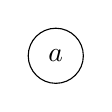
\begin{tikzpicture}
  \ARSnode{a};
\end{tikzpicture}

Normal forms: $a$. Terminating: True. Confluent: True. UNFs: True.

\paragraph{3.\; $A=\{a\},\; R=\{(a,a)\}$}
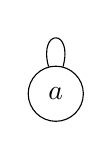
\begin{tikzpicture}
  \ARSnode{a};
  \path (a) edge[loop above] (a);
\end{tikzpicture}

Infinite sequence $a\to a\to\cdots$.  
Terminating: False. Confluent: True. UNFs: False.

\paragraph{4.\; $A=\{a,b,c\},\; R=\{(a,b),(a,c)\}$}
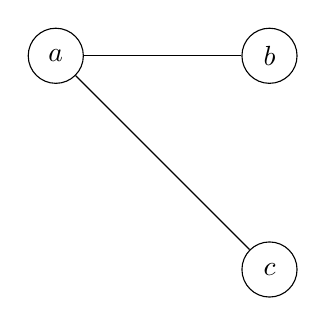
\begin{tikzpicture}[node distance=20mm]
  \ARSnode{a};
  \ARSnodeat{b}{right=of a}
  \ARSnodeat{c}{below=of b}
  \draw (a) edge (b) (a) edge (c);
\end{tikzpicture}

$b$ and $c$ are normal forms, so from $a$ two distinct endpoints are reachable.  
Terminating: True. Confluent: False. UNFs: False.

\paragraph{5.\; $A=\{a,b\},\; R=\{(a,a),(a,b)\}$}
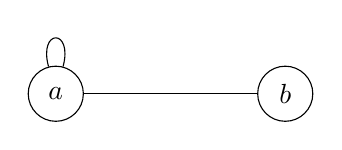
\begin{tikzpicture}[node distance=22mm]
  \ARSnode{a};
  \ARSnodeat{b}{right=of a}
  \draw (a) edge[loop above] (a) (a) edge (b);
\end{tikzpicture}

$b$ is normal; all paths from $a$ can reach $b$.  
Terminating: False. Confluent: True. UNFs: True.

\paragraph{6.\; $A=\{a,b,c\},\; R=\{(a,b),(b,b),(a,c)\}$}
\begin{tikzpicture}[node distance=22mm]
  \ARSnode{a};
  \ARSnodeat{b}{right=of a}
  \ARSnodeat{c}{below=of b}
  \draw (a) edge (b) (a) edge (c) (b) edge[loop above] (b);
\end{tikzpicture}

Non-terminating through $b\to b$; $c$ is normal but unreachable from $b$.  
Terminating: False. Confluent: False. UNFs: False.

\paragraph{7.\; $A=\{a,b,c\},\; R=\{(a,b),(b,b),(a,c),(c,c)\}$}
\begin{tikzpicture}[node distance=22mm]
  \ARSnode{a};
  \ARSnodeat{b}{right=of a}
  \ARSnodeat{c}{below=of b}
  \draw (a) edge (b) (a) edge (c) (b) edge[loop above] (b) (c) edge[loop right] (c);
\end{tikzpicture}

Both $b$ and $c$ loop indefinitely.  
Terminating: False. Confluent: False. UNFs: False.

\textbf{Summary Table:}
\begin{center}
\begin{tabular}{@{}clccc@{}}
\toprule
\# & $(A,R)$ & confluent & terminating & unique NFs \\
\midrule
1 & $(\varnothing,\varnothing)$ & True & True & True \\
2 & $(\{a\},\varnothing)$ & True & True & True \\
3 & $(\{a\},\{(a,a)\})$ & True & False & False \\
4 & $(\{a,b,c\},\{(a,b),(a,c)\})$ & False & True & False \\
5 & $(\{a,b\},\{(a,a),(a,b)\})$ & True & False & True \\
6 & $(\{a,b,c\},\{(a,b),(b,b),(a,c)\})$ & False & False & False \\
7 & $(\{a,b,c\},\{(a,b),(b,b),(a,c),(c,c)\})$ & False & False & False \\
\bottomrule
\end{tabular}
\end{center}

\textbf{All 8 Combinations:}
\begin{center}
\begin{tabular}{@{}ccccl@{}}
\toprule
confluent & terminating & unique NFs & example \\
\midrule
True  & True  & True  & ARS 2 (or 1) \\
True  & True  & False  & \textit{Impossible} \\
True  & False  & True  & ARS 5 \\
True  & False  & False  & ARS 3 \\
False & True  & True  & \textit{Impossible} \\
False & True  & False  & ARS 4 \\
False & False & True  & \textit{Impossible} \\
False & False & False & ARS 6 (or 7) \\
\bottomrule
\end{tabular}
\end{center}

\subsubsection{Questions}
\emph{Is there an easy way to tell from the graph if an ARS will terminate, or do you always have to trace every path?}

% ---------- Week 3 ----------
\subsection{Week 3}

\subsubsection{Notes and Exploration}
Exercises 5 and 5b extended ARS analysis with additional looping rules.

\subsubsection{Homework}
\textbf{Exercise 5.}  
$A=\{a,b\}$ with $a\to a$, $a\to b$.  
Loop $a\to a$ means not terminating, but since all paths eventually lead to $b$, the system is confluent with a unique NF.

\textbf{Exercise 5b.}  
Add $c$ with $a\to c$, $c\to c$.  
Now one branch terminates ($b$) and the other loops, breaking confluence.

\subsubsection{Questions}
\emph{Could we make a version of 5b that still loops but somehow keeps unique normal forms?}

% ---------- Week 4 ----------
\subsection{Week 4}

\subsubsection{Notes and Exploration}
We introduced termination proofs and measure functions.

\subsubsection{Homework}
\paragraph{HW 4.1 (Euclidean Algorithm).}
\begin{verbatim}
while b != 0:
  temp = b
  b = a mod b
  a = temp
return a
\end{verbatim}
This algorithm terminates when $b>0$ because $b$ decreases with each iteration.  
The measure function $m(a,b)=b$ is always non-negative and strictly decreases.

\paragraph{HW 4.2 (Merge Sort).}
\begin{verbatim}
function merge_sort(arr, left, right):
  if left >= right: return
  mid = (left + right) / 2
  merge_sort(arr, left, mid)
  merge_sort(arr, mid+1, right)
  merge(arr, left, mid, right)
\end{verbatim}
The measure $\varphi(left,right)=right-left+1$ decreases with every recursive call.  
When it reaches 1, the recursion stops, proving termination.

\subsubsection{Questions}
\emph{What would it look like to design a sorting algorithm that checks to see if an input is terminating?}

% ---------- Week 5 ----------
\subsection{Week 5}

\subsubsection{Notes and Exploration}
We practiced $\lambda$-calculus reduction and substitution.

\subsubsection{Homework}
Evaluate:
\[
  (\lambda f.\lambda x.f(f(x)))\,(\lambda f.\lambda x.f(f(f(x)))).
\]

\textbf{Step 1.} Parentheses group left:  
\[
  ((\lambda f.\lambda x.f(f(x)))(\lambda f.\lambda x.f(f(f(x))))).
\]

\textbf{Step 2.} Apply $\beta$-reduction:  
\[
  \mapsto \lambda x.(\lambda f.\lambda x.f(f(f(x))))((\lambda f.\lambda x.f(f(f(x))))x).
\]

\textbf{Step 3.} Rename inner $x\to y$ and reduce:  
\[
  (\lambda f.\lambda y.f(f(f(y))))x \mapsto \lambda y.x(x(x(y))).
\]

\textbf{Step 4.} Apply again:  
\[
  \lambda x.\lambda y.x^9(y).
\]

\textbf{Conclusion.}  
The function composes $f$ twice and $f^3$ thrice, resulting in a ninefold application.

\subsubsection{Questions}
\emph{What would happen if we swapped the two functions in the workout?}

% ---------- Week 6 ----------
\subsection{Week 6}

\subsubsection{Notes and Exploration}
We computed factorial using the fixed-point combinator \texttt{fix}.

\subsubsection{Homework}
Compute:
\[
\texttt{let rec fact = \textbackslash n. if n=0 then 1 else n * fact (n-1) in 3}
\]
Using the rules:
\[
\texttt{fix F $\mapsto$ F (fix F)}, \quad
\texttt{let rec f = e1 in e2 $\mapsto$ let f = (fix (\textbackslash f.e1)) in e2}.
\]
We unfold recursively:
\[
\texttt{fact 3 $\mapsto$ 3 * (fix F) 2 $\mapsto$ 3 * 2 * 1 = 6}.
\]

\textbf{Conclusion.}  
Following only the allowed computation rules, \texttt{fact 3} reduces to \textbf{6}.

\subsubsection{Questions}
\emph{Would using $\alpha$-conversion anywhere in the factorial example change the result, or just make it cleaner?}

% ---------- Week 7 ----------
\subsection{Week 7}

\subsubsection{Notes and Exploration}
Parsing and context-free grammars. We use the grammar (nonterminals \texttt{Exp}, \texttt{Exp1}, \texttt{Exp2}):

\begin{verbatim}
Exp  -> Exp '+' Exp1
Exp1 -> Exp1 '*' Exp2
Exp2 -> Integer
Exp2 -> '(' Exp ')'
Exp  -> Exp1
Exp1 -> Exp2
\end{verbatim}

\subsubsection{Homework: Parse Trees}
Below are derivation trees (concrete syntax trees) for the required expressions. 
Nonterminals are boxed; terminals are leaves.

\paragraph{(a) \texttt{2+1}}
\begin{center}
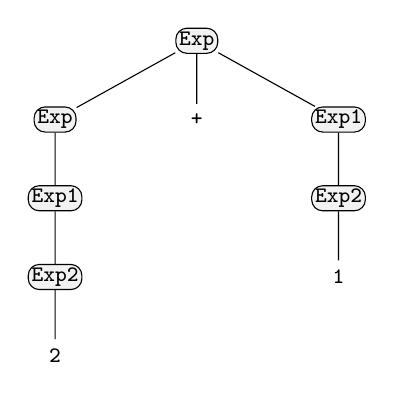
\begin{tikzpicture}[ptree]
\node[nt]{Exp}
  child { node[nt]{Exp}
    child { node[nt]{Exp1}
      child { node[nt]{Exp2}
        child { node[tm]{2} }
      }
    }
  }
  child { node[tm]{+} }
  child { node[nt]{Exp1}
    child { node[nt]{Exp2}
      child { node[tm]{1} }
    }
  };
\end{tikzpicture}
\end{center}

\paragraph{(b) \texttt{1+2*3}}
\begin{center}
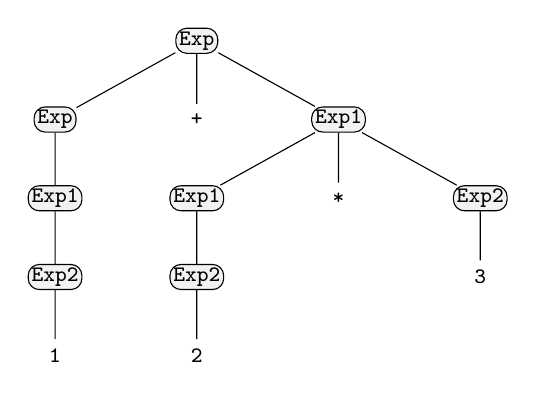
\begin{tikzpicture}[ptree]
\node[nt]{Exp}
  child { node[nt]{Exp}
    child { node[nt]{Exp1}
      child { node[nt]{Exp2}
        child { node[tm]{1} }
      }
    }
  }
  child { node[tm]{+} }
  child { node[nt]{Exp1}
    child { node[nt]{Exp1}
      child { node[nt]{Exp2} child { node[tm]{2} } }
    }
    child { node[tm]{*} }
    child { node[nt]{Exp2} child { node[tm]{3} } }
  };
\end{tikzpicture}
\end{center}

\paragraph{(c) \texttt{1+(2*3)}}
\begin{center}
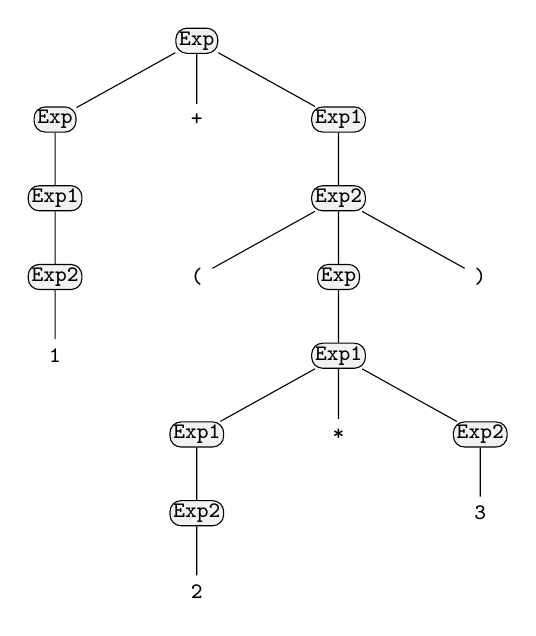
\begin{tikzpicture}[ptree]
\node[nt]{Exp}
  child { node[nt]{Exp}
    child { node[nt]{Exp1}
      child { node[nt]{Exp2} child { node[tm]{1} } }
    }
  }
  child { node[tm]{+} }
  child { node[nt]{Exp1}
    child { node[nt]{Exp2}
      child { node[tm]{(} }
      child { node[nt]{Exp}
        child { node[nt]{Exp1}
          child { node[nt]{Exp1}
            child { node[nt]{Exp2} child { node[tm]{2} } }
          }
          child { node[tm]{*} }
          child { node[nt]{Exp2} child { node[tm]{3} } }
        }
      }
      child { node[tm]{)} }
    }
  };
\end{tikzpicture}
\end{center}


\paragraph{(d) \texttt{(1+2)*3}}
\begin{center}
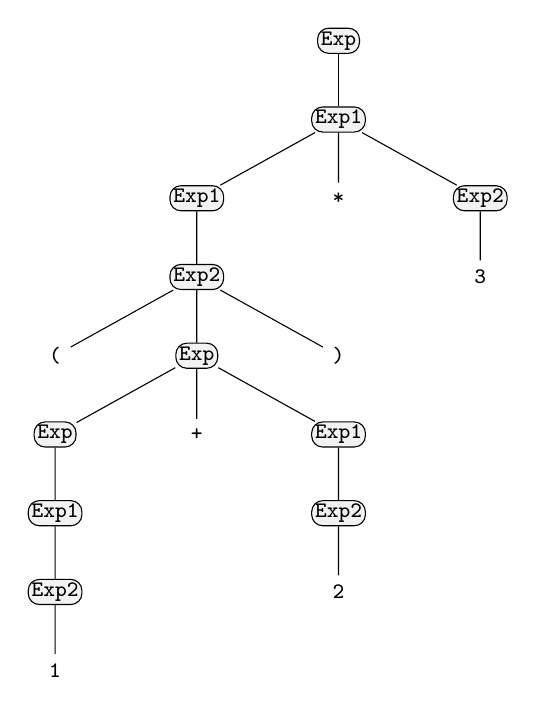
\begin{tikzpicture}[ptree]
\node[nt]{Exp}
  child { node[nt]{Exp1}
    child { node[nt]{Exp1}
      child { node[nt]{Exp2}
        child { node[tm]{(} }
        child { node[nt]{Exp}
          child { node[nt]{Exp}
            child { node[nt]{Exp1}
              child { node[nt]{Exp2} child { node[tm]{1} } }
            }
          }
          child { node[tm]{+} }
          child { node[nt]{Exp1}
            child { node[nt]{Exp2} child { node[tm]{2} } }
          }
        }
        child { node[tm]{)} }
      }
    }
    child { node[tm]{*} }
    child { node[nt]{Exp2} child { node[tm]{3} } }
  };
\end{tikzpicture}
\end{center}

\paragraph{(e) \texttt{1+2*3+4*5+6}}
\begin{center}
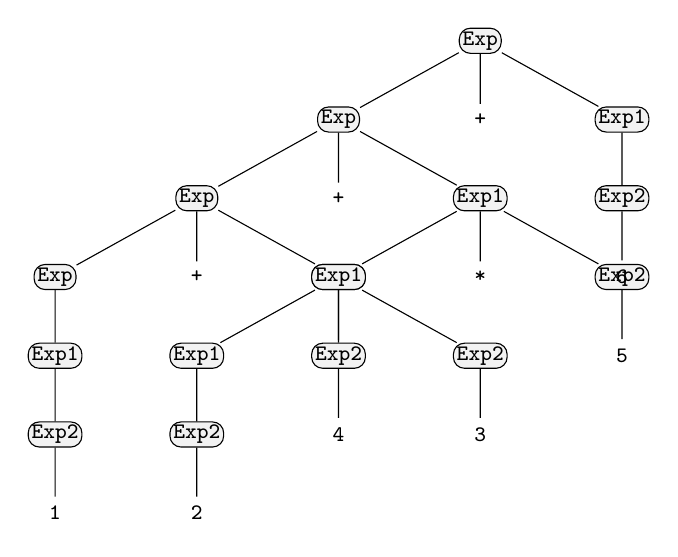
\begin{tikzpicture}[ptree]
\node[nt]{Exp}
  % Left: ((1 + 2*3) + 4*5)
  child { node[nt]{Exp}
    child { node[nt]{Exp}
      % (1 + 2*3)
      child { node[nt]{Exp}
        child { node[nt]{Exp1}
          child { node[nt]{Exp2} child { node[tm]{1} } }
        }
      }
      child { node[tm]{+} }
      child { node[nt]{Exp1}
        child { node[nt]{Exp1}
          child { node[nt]{Exp2} child { node[tm]{2} } }
        }
        child { node[tm]{*} }
        child { node[nt]{Exp2} child { node[tm]{3} } }
      }
    }
    child { node[tm]{+} }
    child { node[nt]{Exp1}
      child { node[nt]{Exp1}
        child { node[nt]{Exp2} child { node[tm]{4} } }
      }
      child { node[tm]{*} }
      child { node[nt]{Exp2} child { node[tm]{5} } }
    }
  }
  child { node[tm]{+} }
  child { node[nt]{Exp1}
    child { node[nt]{Exp2} child { node[tm]{6} } }
  };
\end{tikzpicture}
\end{center}

% =========================================================
\subsubsection{Questions}
\emph{Could this grammar still work if “+” and “” had the same priority?}

% ---------- Week 8 ----------
\subsection{Week 8}

\subsubsection{Notes and Exploration}
I completed Levels 5--8 of the \emph{Natural Number Game} (NNG). The key tools were:
\begin{itemize}[leftmargin=1.4em]
  \item \textbf{Rewriting} with \texttt{rw [lemma]} to substitute equals for equals.
  \item \textbf{\texttt{rfl}} to close a goal when both sides are definitionally identical.
  \item Peano-style equations for addition and numerals, including \texttt{add\_zero}, \texttt{add\_succ}, \texttt{add\_one}, \texttt{one\_eq\_succ\_zero}, and \texttt{two\_eq\_succ\_one}.
\end{itemize}

\subsubsection{Homework (NNG Levels 5--8)}
\paragraph{5/8: Adding zero.} \emph{Goal:} $a + (b+0) + (c+0) = a+b+c$.\\
\emph{Lean steps:} \texttt{rw [add\_zero]} (on $b+0$), \texttt{rw [add\_zero]} (on $c+0$), \texttt{rfl}.

\paragraph{6/8: Precision rewriting.} \emph{Goal:} $a + (b+0) + (c+0) = a+b+c$.\\
\emph{Lean steps:} \texttt{rw [add\_zero]} (on $b+0$), \texttt{rw [add\_zero]} (on $c+0$), \texttt{rfl}.

\paragraph{7/8: \texttt{add\_succ}.} \emph{Goal:} $\mathrm{succ}\,n = n+1$.\\
\emph{Lean steps:} \texttt{rw [one\_eq\_succ\_zero]} to get $n+1=n+\mathrm{succ}\,0$; \texttt{rw [add\_succ]} to obtain $\mathrm{succ}(n+0)$; \texttt{rw [add\_zero]}; \texttt{rfl}.

\paragraph{8/8: $2+2=4$.} \emph{Outline:} Rewrite $2$ and $4$ as successors (\texttt{two\_eq\_succ\_one}, etc.), use \texttt{add\_succ} to pull \(\mathrm{succ}\) out of addition stepwise, and finish by \texttt{rfl} once both sides match.

\subsubsection{Natural-Language Proof (English math proof)}
\paragraph{Claim.} \(2+2=4\).

\paragraph{Assumptions/Definitions.}
Let \(0\) be the base natural number and \(\mathrm{succ}(n)\) the successor of \(n\).
Define \(1=\mathrm{succ}(0)\), \(2=\mathrm{succ}(1)\), and \(4=\mathrm{succ}(\mathrm{succ}(\mathrm{succ}(\mathrm{succ}(0))))\).
Addition is defined by the Peano axioms:
\[
\forall a,\; a+0=a \quad\text{and}\quad \forall a,b,\; a+\mathrm{succ}(b)=\mathrm{succ}(a+b).
\]

\paragraph{Proof.}
We compute \(2+2\) using the addition axioms.
First rewrite \(2=\mathrm{succ}(1)\), so
\[
2+2 \;=\; 2+\mathrm{succ}(1) \;=\; \mathrm{succ}(2+1) \quad\text{(by the second axiom).}
\]
Again rewrite \(1=\mathrm{succ}(0)\) to get
\[
2+1 \;=\; 2+\mathrm{succ}(0) \;=\; \mathrm{succ}(2+0) \;=\; \mathrm{succ}(2) \quad\text{(using both axioms).}
\]
Therefore
\[
2+2 \;=\; \mathrm{succ}(2+1) \;=\; \mathrm{succ}(\mathrm{succ}(2)).
\]
Since \(2=\mathrm{succ}(1)\), we have
\[
\mathrm{succ}(\mathrm{succ}(2))=\mathrm{succ}(\mathrm{succ}(\mathrm{succ}(1)))=
\mathrm{succ}(\mathrm{succ}(\mathrm{succ}(\mathrm{succ}(0))))=4.
\]
Hence \(2+2=4\). \(\square\)

\subsubsection{Discord Question}
\emph{When using \texttt{rw [add\_zero]}, how does Lean know which part of the equation to rewrite first?}

% ---------- Week 9 ----------
\subsection{Week 9}

\subsubsection{Notes and Exploration}
This week I worked through \emph{Addition World} in the Natural Number Game.  
Key theorems proved in this world:
\begin{itemize}[leftmargin=1.4em]
  \item \textbf{zero\_add:} $0 + n = n$ (proved by induction).
  \item \textbf{succ\_add:} $\mathrm{succ}(a) + b = \mathrm{succ}(a + b)$ (proved by induction).
  \item \textbf{add\_comm:} $a + b = b + a$ (commutativity of $+$).
  \item \textbf{add\_assoc:} $(a + b) + c = a + (b + c)$ (associativity of $+$).
  \item \textbf{add\_right\_comm:} $(a + b) + c = (a + c) + b$.
\end{itemize}

The HW 9 instruction is:  
For Level 5 of addition world (\texttt{add\_right\_comm}), give two solutions in the report:
(1) a proof that uses induction and  
(2) a proof that does \emph{not} use induction.  
For each version, also write the corresponding ``pen-and-paper'' math proof.

\subsubsection{Homework (Addition World Level 5 / HW 9)}

\paragraph{Theorem (Level 5).}
For all natural numbers $a,b,c$, we have
\[
(a + b) + c \;=\; (a + c) + b.
\]
In Lean, this theorem is called \texttt{add\_right\_comm}.

\bigskip
\noindent\textbf{Solution A: With Induction.}  
We prove \texttt{add\_right\_comm} by induction on $c$.

\emph{Lean tactic steps:}
\begin{itemize}[leftmargin=1.4em]
  \item \texttt{induction c with d hd}
  \item \texttt{rw [add\_zero]}
  \item \texttt{rw [add\_zero]}
  \item \texttt{rfl}
  \item \texttt{rw [add\_succ]}
  \item \texttt{rw [succ\_add]}
  \item \texttt{rw [hd]}
  \item \texttt{rfl}
\end{itemize}

Explanation of structure (what the tactics are doing, summarized in math terms):

\emph{Base case ($c=0$).}  
Goal:
\[
(a+b)+0 \;=\; (a+0)+b.
\]
By \texttt{add\_zero}, $(a+b)+0 = a+b$, and $(a+0)+b = a+b$.  
So both sides are $a+b$. Closed by \texttt{rfl}.

\emph{Inductive step ($c = \mathrm{succ}(d)$).}  
Induction hypothesis (called \texttt{hd} in Lean):
\[
(a+b)+d \;=\; (a+d)+b.
\]
Goal:
\[
(a+b)+\mathrm{succ}(d) \;=\; (a+\mathrm{succ}(d))+b.
\]

Using the Peano definition of $+$ on the right argument,
\[
(a+b)+\mathrm{succ}(d) = \mathrm{succ}((a+b)+d)
\quad\text{and}\quad
a+\mathrm{succ}(d) = \mathrm{succ}(a+d).
\]
So the right-hand side becomes
\[
(a+\mathrm{succ}(d))+b
= (\mathrm{succ}(a+d))+b
= \mathrm{succ}\big((a+d)+b\big)
\]
using \texttt{succ\_add}, which says $\mathrm{succ}(x)+y=\mathrm{succ}(x+y)$.

Thus the goal reduces to
\[
\mathrm{succ}\big((a+b)+d\big)
=
\mathrm{succ}\big((a+d)+b\big).
\]
By the induction hypothesis, $(a+b)+d = (a+d)+b$, so the two $\mathrm{succ}(\cdot)$ terms are equal. This closes with \texttt{rfl}.

\emph{Conclusion.}  
By induction on $c$, $(a+b)+c = (a+c)+b$ holds for all $a,b,c$.

\bigskip
\noindent\textbf{Solution B: Without Induction.}  
We can also prove \texttt{add\_right\_comm} using only associativity and commutativity of addition, without \texttt{induction}.

\emph{Lean tactic steps (no induction):}
\begin{itemize}[leftmargin=1.4em]
  \item \texttt{rw [add\_assoc]}
  \item \texttt{rw [add\_comm b c]}
  \item \texttt{rw [\textbackslash leftarrow{} add\_assoc]}
  \item \texttt{rfl}
\end{itemize}

Those steps correspond exactly to the following algebra moves:
\[
(a+b)+c
\;=\;
a+(b+c)
\quad\text{(associativity, \texttt{add\_assoc})}
\]
\[
=\;
a+(c+b)
\quad\text{(commutativity on $b+c$, \texttt{add\_comm b c})}
\]
\[
=\;
(a+c)+b
\quad\text{(associativity again, undoing \texttt{add\_assoc})}.
\]
This matches the goal $(a+b)+c = (a+c)+b$.

\bigskip
\noindent\textbf{English/Pen-and-Paper Proofs for HW 9}

\paragraph{Solution A (Induction Proof in Math).}
We prove $(a+b)+c = (a+c)+b$ for all $a,b,c \in \mathbb{N}$ by induction on $c$.

\textbf{Base case:} $c=0$.  
Then
\[
(a+b)+0 = a+b
\quad\text{and}\quad
(a+0)+b = a+b,
\]
because $x+0=x$ for any $x$.  
So $(a+b)+0 = (a+0)+b$.

\textbf{Inductive step:} Assume $(a+b)+d = (a+d)+b$ for some $d$.  
We must show $(a+b)+\mathrm{succ}(d) = (a+\mathrm{succ}(d))+b$.

By the Peano definition of addition on the right argument,
\[
(a+b)+\mathrm{succ}(d) = \mathrm{succ}((a+b)+d).
\]
Also,
\[
a+\mathrm{succ}(d) = \mathrm{succ}(a+d),
\]
so
\[
(a+\mathrm{succ}(d))+b 
= (\mathrm{succ}(a+d))+b 
= \mathrm{succ}((a+d)+b),
\]
using the lemma $\mathrm{succ}(x)+y = \mathrm{succ}(x+y)$.

So it suffices to show
\[
\mathrm{succ}((a+b)+d) = \mathrm{succ}((a+d)+b),
\]
which follows from the induction hypothesis $(a+b)+d = (a+d)+b$.  
Therefore the statement holds for $\mathrm{succ}(d)$.

By induction on $c$, $(a+b)+c = (a+c)+b$ for all $a,b,c$.

\paragraph{Solution B (Algebraic / No Induction).}
We use associativity and commutativity of addition on $\mathbb{N}$.

Starting from the left-hand side,
\[
(a+b)+c = a+(b+c)
\quad\text{(associativity of $+$)},
\]
\[
= a+(c+b)
\quad\text{(commutativity of $+$)},
\]
\[
= (a+c)+b
\quad\text{(associativity of $+$ again)}.
\]
This is exactly the desired right-hand side $(a+c)+b$.  
No induction was needed.

\subsubsection{Questions}
\emph{When should I solve these problems using induction vs without?}

% ---------- Week 10 ----------
\subsection{Week 10}

\subsubsection{Notes and Exploration}
This week I finished the \textbf{Lean Logic Game} tutorial on implications, called \emph{Party Snacks}. The tutorial shows that
\begin{itemize}[leftmargin=1.4em]
  \item an implication $P \to Q$ is a function from evidence of $P$ to evidence of $Q$;
  \item conjunction $P \land Q$ is a pair made with \texttt{and\_intro};
  \item taking a function of \emph{two} inputs and turning it into a function of \emph{one} input that returns a function (currying) is exactly what Lean is doing when we write \texttt{fun x => fun y => ...}.
\end{itemize}
Levels 6--9 are the ones required for the HW, so below I spell out every little step.

\subsubsection{Homework (Party Snacks, Levels 6--9)}

% ---------------- Level 6 ----------------
\paragraph{Level 6/9 (\texttt{and\_imp}).}
\textbf{Goal.} Build
\[
C \to D \to S
\]
from the assumption
\[
h : C \land D \to S.
\]

So Lean is asking us to produce a \emph{function} that, when you hand it a $c : C$ and then a $d : D$, it can call $h$ on the \emph{pair} $(c,d)$ and get an $S$.

\textbf{Plan.}
\begin{enumerate}[label=\arabic*.,leftmargin=1.4em]
  \item Start a function that takes $c : C$.
  \item Inside it, start another function that takes $d : D$.
  \item Turn $(c,d)$ into evidence of $C \land D$ using \texttt{and\_intro c d}.
  \item Feed that to $h$ to get the $S$.
\end{enumerate}

\textbf{Step-by-step term.}
\[
\underbrace{\texttt{fun c : C =>}}_{\text{1st argument}}
\underbrace{\texttt{ fun d : D =>}}_{\text{2nd argument}}
\underbrace{\texttt{ h (and\_intro c d) }}_{\text{call the given implication}}
\]

\textbf{What Lean checks.}
\begin{itemize}[leftmargin=1.4em]
  \item After \texttt{fun c =>} the goal becomes $D \to S$ (because we promised to produce a function of $c$).
  \item After \texttt{fun d =>} the goal becomes $S$.
  \item \texttt{and\_intro c d} has type $C \land D$.
  \item $h$ has type $C \land D \to S$, so $h (and\_intro c d)$ has type $S$, which matches the goal.
\end{itemize}

\textbf{Final Lean line.}
\begin{verbatim}
exact fun c => fun d => h (and_intro c d)
\end{verbatim}

% ---------------- Level 7 ----------------
\paragraph{Level 7/9 (\texttt{and\_imp 2}).}
\textbf{Goal.} Build
\[
(C \land D) \to S
\]
from the assumption
\[
h : C \to D \to S.
\]

This is the \emph{uncurried} direction: instead of receiving $C$ and $D$ separately, we receive \emph{one} thing, namely evidence for $C \land D$, and from that we must produce $S$.

\textbf{Plan.}
\begin{enumerate}[label=\arabic*.,leftmargin=1.4em]
  \item Start a function that takes $hcd : C \land D$.
  \item From $hcd$ we can project the left part: \texttt{hcd.left} has type $C$.
  \item From $hcd$ we can project the right part: \texttt{hcd.right} has type $D$.
  \item Since $h : C \to D \to S$, we can first give it a $C$, then a $D$, to get $S$: \texttt{h (hcd.left) (hcd.right)}.
\end{enumerate}

\textbf{Step-by-step term.}
\[
\texttt{fun hcd : C ∧ D =>}
\quad
\texttt{h hcd.left hcd.right}
\]

\textbf{What Lean checks.}
\begin{itemize}[leftmargin=1.4em]
  \item After \texttt{fun hcd =>} the goal is $S$.
  \item \texttt{hcd.left} : $C$, \texttt{hcd.right} : $D$.
  \item \texttt{h hcd.left} : $D \to S$.
  \item \texttt{(h hcd.left) hcd.right} : $S$.
\end{itemize}

\textbf{Final Lean line.}
\begin{verbatim}
exact fun hcd => h hcd.left hcd.right
\end{verbatim}

% ---------------- Level 8 ----------------
\paragraph{Level 8/9 (\texttt{Distribute}).}
\textbf{Given.}
\[
h : (S \to C) \land (S \to D)
\]
So $h.left$ has type $S \to C$ and $h.right$ has type $S \to D$.

\textbf{Goal.}
\[
S \to C \land D
\]
i.e. “if we have an $s : S$, we can produce both a $C$ and a $D$.”

\textbf{Plan.}
\begin{enumerate}[label=\arabic*.,leftmargin=1.4em]
  \item Start a function that takes $s : S$.
  \item Use $h.left : S \to C$ and apply it to $s$ to get a $C$.
  \item Use $h.right : S \to D$ and apply it to $s$ to get a $D$.
  \item Glue those two into $C \land D$ using \texttt{and\_intro}.
\end{enumerate}

\textbf{Step-by-step term.}
\[
\texttt{fun s : S =>}
\quad
\texttt{and\_intro (h.left s) (h.right s)}
\]

\textbf{What Lean checks.}
\begin{itemize}[leftmargin=1.4em]
  \item After \texttt{fun s =>} the goal is $C \land D$.
  \item \texttt{h.left s} : $C$, \texttt{h.right s} : $D$.
  \item \texttt{and\_intro (h.left s) (h.right s)} : $C \land D$.
\end{itemize}

\textbf{Final Lean line.}
\begin{verbatim}
exact fun s => and_intro (h.left s) (h.right s)
\end{verbatim}

% ---------------- Level 9 ----------------
\paragraph{Level 9/9 (\texttt{Uncertain Snacks}, boss).}
\textbf{Goal.}
\[
R \to (S \to R) \land (\neg S \to R).
\]
Read: “If Riffin is bringing a snack, then (1) if Sybeth brings one, Riffin is bringing a snack, and (2) if Sybeth does \emph{not} bring one, Riffin is still bringing a snack.”

\textbf{Given.}
We start only with $r : R$.

\textbf{Plan.}
\begin{enumerate}[label=\arabic*.,leftmargin=1.4em]
  \item Start a function that takes $r : R$.
  \item We must output an \emph{and}-pair, so we will finish with \texttt{and\_intro ... ...}.
  \item Left part of the pair must have type $S \to R$.
  \item Right part of the pair must have type $(\neg S) \to R$.
  \item But we already have $r : R$, and neither of these two subgoals actually needs their argument.
  \item So for the left part we write \texttt{fun \_ : S => r}.
  \item For the right part we write \texttt{fun \_ : ¬ S => r}.
\end{enumerate}

\textbf{Step-by-step term.}
\[
\texttt{fun r : R =>}
\quad
\texttt{and\_intro}
\quad
  \underbrace{\texttt{(fun \_ : S => r)}}_{\text{has type } S \to R}
\quad
  \underbrace{\texttt{(fun \_ : ¬ S => r)}}_{\text{has type } ¬S \to R}
\]

\textbf{What Lean checks.}
\begin{itemize}[leftmargin=1.4em]
  \item After \texttt{fun r =>} the goal is $(S \to R) \land (\neg S \to R)$.
  \item \texttt{fun \_ => r} always has the right implication type, because no matter what you give it, it returns $r : R$.
  \item \texttt{and\_intro (fun \_ => r) (fun \_ => r)} has the desired conjunction type.
\end{itemize}

\textbf{Final Lean line.}
\begin{verbatim}
exact fun r => and_intro (fun _ => r) (fun _ => r)
\end{verbatim}

\subsubsection{Questions}
\emph{When is it better to package information together, and when is it better to keep it separate?}

% ---------- Week 11 ----------
\subsection{Week 11}

\subsubsection{Notes and Exploration}
I completed Levels 9--12 of the \emph{Lean Logic Negation Tutorial}. The key ideas are:
\begin{itemize}[leftmargin=1.4em]
  \item \(\neg P\) is shorthand for \(P \to \mathrm{False}\).
  \item From a conjunction \(P \land Q\), we project with \texttt{.left} and \texttt{.right}.
  \item \texttt{false\_elim} proves any proposition from \(\mathrm{False}\) (principle of explosion).
\end{itemize}

\subsubsection{Homework (Negation Tutorial Levels 9--12)}

% ---------------- Level 9 ----------------
\paragraph{Level 9/12: \textit{Allergy \#1} (\(\neg(P \land A)\) from \(h : P \to \neg A\)).}
\textbf{Goal.} \(\neg(P \land A)\). \quad
\textbf{Given.} \(h : P \to \neg A\).
\begin{itemize}[leftmargin=1.4em]
  \item Assume \(hpa : P \land A\). Then \(hpa.left : P\) and \(hpa.right : A\).
  \item From \(h\) we get \(h\,hpa.left : \neg A\), i.e.\ \(A \to \mathrm{False}\).
  \item Apply to \(hpa.right\) to reach \(\mathrm{False}\).
\end{itemize}
\textbf{Final Lean line.}
\begin{verbatim}
exact (fun hpa => (h hpa.left) hpa.right)
\end{verbatim}

% ---------------- Level 10 ----------------
\paragraph{Level 10/12: \textit{Allergy \#2} (\(P \to \neg A\) from \(h : \neg(P \land A)\)).}
\textbf{Goal.} \(P \to (A \to \mathrm{False})\). \quad
\textbf{Given.} \(h : \neg(P \land A)\).
\begin{itemize}[leftmargin=1.4em]
  \item Take \(p:P\) and \(a:A\); then \(\langle p,a\rangle : P \land A\).
  \item Apply \(h\) to derive \(\mathrm{False}\).
\end{itemize}
\textbf{Final Lean line.}
\begin{verbatim}
exact (fun p a => h ⟨p, a⟩)
\end{verbatim}

% ---------------- Level 11 ----------------
\paragraph{Level 11/12: \textit{not\_not\_not} (\(\neg A\) from \(h : \neg\neg\neg A\)).}
\textbf{Goal.} \(\neg A\). \quad
\textbf{Given.} \(h : (\neg\neg A) \to \mathrm{False}\).
\begin{itemize}[leftmargin=1.4em]
  \item To show \(A \to \mathrm{False}\), assume \(a:A\).
  \item Build \(\neg\neg A\) by \((\lambda na:\neg A,\, na\,a)\).
  \item Feed this into \(h\) to get \(\mathrm{False}\).
\end{itemize}
\textbf{Final Lean line.}
\begin{verbatim}
exact (fun a => h (fun na => na a))
\end{verbatim}

% ---------------- Level 12 ----------------
\paragraph{Level 12/12 (Boss): \(\neg\neg B\) from \(h : \neg(B \to C)\).}
\textbf{Goal.} \(\neg\neg B\), i.e.\ \((\neg B) \to \mathrm{False}\). \quad
\textbf{Given.} \(h : (B \to C) \to \mathrm{False}\).
\begin{itemize}[leftmargin=1.4em]
  \item Assume \(nb : \neg B\). Define \(f : B \to C\) by \(f\,b := \texttt{false\_elim}(nb\,b)\).
  \item Then \(h\,f : \mathrm{False}\). Hence \((\neg B) \to \mathrm{False}\).
\end{itemize}
\textbf{Final Lean line.}
\begin{verbatim}
exact (fun nb => h (fun b => false_elim (nb b)))
\end{verbatim}

\subsubsection{Questions}
\emph{Is there a quick rule of thumb for spotting when a goal is really “prove a function to False”?}

% ---------- Week 12 ----------
\subsection{Week 12}

\subsubsection{Notes and Exploration}
We read the Towers of Hanoi notes and treated the recursive definition of \texttt{hanoi} as a pair of rewrite rules.  
The two rules are

\[
\texttt{hanoi 1 x y = move x y}
\]
\[
\texttt{hanoi (n+1) x y =}
\quad
\texttt{hanoi n x (other x y);}
\quad
\texttt{move x y;}
\quad
\texttt{hanoi n (other x y) y.}
\]

I tried to think of \texttt{hanoi n x y} as the phrase “move a tower of size \(n\) from peg \(x\) to peg \(y\) using the remaining peg.”  
The trace then becomes a long horizontal and vertical picture of the recursive calls, where indentation shows call depth and each \texttt{move} line is an actual step in time.

\subsubsection{Homework (Towers of Hanoi)}

\paragraph{1. Completed execution for \texttt{hanoi 5 0 2}.}

\begin{verbatim}
hanoi 5 0 2
  hanoi 4 0 1
    hanoi 3 0 2
      hanoi 2 0 1
        hanoi 1 0 2 = move 0 2
        move 0 1
        hanoi 1 2 1 = move 2 1
      move 0 2
      hanoi 2 1 2
        hanoi 1 1 0 = move 1 0
        move 1 2
        hanoi 1 0 2 = move 0 2
    move 0 1
    hanoi 3 2 1
      hanoi 2 2 0
        hanoi 1 2 1 = move 2 1
        move 2 0
        hanoi 1 1 0 = move 1 0
      move 2 1
      hanoi 2 0 1
        hanoi 1 0 2 = move 0 2
        move 0 1
        hanoi 1 2 1 = move 2 1
  move 0 2
  hanoi 4 1 2
    hanoi 3 1 0
      hanoi 2 1 2
        hanoi 1 1 0 = move 1 0
        move 1 2
        hanoi 1 0 2 = move 0 2
      move 1 0
      hanoi 2 2 0
        hanoi 1 2 1 = move 2 1
        move 2 0
        hanoi 1 1 0 = move 1 0
    move 1 2
    hanoi 3 0 2
      hanoi 2 0 1
        hanoi 1 0 2 = move 0 2
        move 0 1
        hanoi 1 2 1 = move 2 1
      move 0 2
      hanoi 2 1 2
        hanoi 1 1 0 = move 1 0
        move 1 2
        hanoi 1 0 2 = move 0 2
\end{verbatim}

Every time the rule for \(\texttt{hanoi (n+1) x y}\) fires, the trace splits into a smaller call that uses the helper peg, then a single \texttt{move}, then another smaller call that finishes the job.

\paragraph{2. Moves extracted from the trace.}

Reading only the \texttt{move} lines from top to bottom gives the sequence of moves that solves the puzzle with five disks, from peg \(0\) to peg \(2\):

\begin{enumerate}[leftmargin=1.4em]
  \item move disk from peg 0 to peg 2
  \item move disk from peg 0 to peg 1
  \item move disk from peg 2 to peg 1
  \item move disk from peg 0 to peg 2
  \item move disk from peg 1 to peg 0
  \item move disk from peg 1 to peg 2
  \item move disk from peg 0 to peg 2
  \item move disk from peg 0 to peg 1
  \item move disk from peg 2 to peg 1
  \item move disk from peg 2 to peg 0
  \item move disk from peg 1 to peg 0
  \item move disk from peg 2 to peg 1
  \item move disk from peg 0 to peg 2
  \item move disk from peg 0 to peg 1
  \item move disk from peg 2 to peg 1
  \item move disk from peg 0 to peg 2
  \item move disk from peg 1 to peg 0
  \item move disk from peg 1 to peg 2
  \item move disk from peg 0 to peg 2
  \item move disk from peg 1 to peg 0
  \item move disk from peg 2 to peg 1
  \item move disk from peg 2 to peg 0
  \item move disk from peg 1 to peg 0
  \item move disk from peg 1 to peg 2
  \item move disk from peg 0 to peg 2
  \item move disk from peg 0 to peg 1
  \item move disk from peg 2 to peg 1
  \item move disk from peg 0 to peg 2
  \item move disk from peg 1 to peg 0
  \item move disk from peg 1 to peg 2
  \item move disk from peg 0 to peg 2
\end{enumerate}

There are \(2^{5}-1 = 31\) moves, which matches the usual formula for the minimal number of moves with five disks.

\paragraph{3. Online verification.}

I checked this list of moves against the interactive Towers of Hanoi link from the notes.  
Entering the moves in order really does move the entire stack of five disks from peg \(0\) to peg \(2\) without ever placing a larger disk on top of a smaller one, and the game also reports that the puzzle was solved in thirty one moves.  
So the completed execution trace and the extracted move list are consistent with the online version.

\subsubsection{Questions}
\emph{How can I formally prove that the Towers of Hanoi algorithm always takes exactly two to the n minus one moves?}

% ---------- Week 13 ----------
\subsection{Week 13}

\subsubsection{Notes and Exploration}
In the Hanoi notes, we treated the recursive definition of \texttt{hanoi} as two rewrite rules:
\[
\texttt{hanoi 1 x y = move x y}
\]
\[
\texttt{hanoi (n+1) x y =}
\quad
\texttt{hanoi n x (other x y);}
\quad
\texttt{move x y;}
\quad
\texttt{hanoi n (other x y) y.}
\]
To prove the move-count formula, the key idea is: \emph{count how many \texttt{move} lines these rewrite rules generate.}
This naturally gives a recurrence, and then we solve it by induction.

\subsubsection{Homework}

\textbf{Claim.}  
Let $T(n)$ be the number of \texttt{move} commands produced by the trace of \texttt{hanoi n x y} (for any pegs $x,y$).  
Then for all $n \ge 1$,
\[
T(n) = 2^{n}-1.
\]

\textbf{Step 1 (Base case from the rewrite rule).}  
For $n=1$, the rule says:
\[
\texttt{hanoi 1 x y = move x y.}
\]
So the trace has exactly one \texttt{move} line. Therefore
\[
T(1)=1,
\]
and this matches the formula because $2^{1}-1=1$.

\textbf{Step 2 (Build the recurrence by counting moves in the second rule).}  
For $n+1$, the rule expands \texttt{hanoi (n+1) x y} into three parts:
\begin{enumerate}[leftmargin=1.4em]
  \item \texttt{hanoi n x (other x y)} \quad contributes $T(n)$ moves,
  \item \texttt{move x y} \quad contributes $1$ move,
  \item \texttt{hanoi n (other x y) y} \quad contributes $T(n)$ moves.
\end{enumerate}
So the total number of moves is
\[
T(n+1)=T(n)+1+T(n)=2T(n)+1.
\]

\textbf{Step 3 (Induction proof).}  
We prove $T(n)=2^{n}-1$ for all $n\ge 1$ by induction on $n$.

\emph{Base case ($n=1$).}  
Already shown: $T(1)=1=2^{1}-1$.

\emph{Inductive step.}  
Assume as the induction hypothesis that for some $n\ge 1$,
\[
T(n)=2^{n}-1.
\]
Using the recurrence from Step 2,
\[
T(n+1)=2T(n)+1.
\]
Substitute the hypothesis:
\[
T(n+1)=2(2^{n}-1)+1=2^{n+1}-2+1=2^{n+1}-1.
\]
This is exactly the desired formula for $n+1$.

\textbf{Conclusion.}  
By induction, for every $n\ge 1$, the trace of \texttt{hanoi n x y} contains exactly $2^{n}-1$ \texttt{move} lines.

\subsubsection{Questions}
\emph{Does it matter which pegs are called 0,1,2, or is the move count always the same?}

% =========================================================
\section{Essay (Synthesis)}
This section intentionally left blank.

% =========================================================
\section{Evidence of Participation}
This section intentionally left blank.

% =========================================================
\section{Conclusion}
This section intentionally left blank.

% =========================================================
\section*{References}

\end{document}
